In this chapter we briefly introduce the major principles of
gravitational wave astronomy.  We start in
section~\ref{sec:general_relativity} with a review of general
relativity, starting from the relevant mathematics.  In
section~\ref{sec:gravitational_radiation} we show how general
relativity predicts the existence of gravitational radiation and
discuss some of the properties of this radiation.  Then in
section~\ref{sec:effects_of_waves} we show how gravitational radiation
affects freely-falling particles.  This motivates the nature of the
LIGO experiment to search for gravitational waves, an overview of the
LIGO detectors is given in section~\ref{sec:ligo_detectors}.

\section{General Relativity}
\label{sec:general_relativity}

We start with an overview of differential geometry and build to
Einstein's equations.  This is of necessity very brief, readers are
referred to the textbooks by Misner, Thorne and Wheeler~\cite{MTW} and
Carroll~\cite{carrollTextbook} for more complete treatments.

\subsection{Elements of differential geometry}

An $n$-dimensional ($C^\infty$) manifold $\mathcal{M}$ is a set of
points plus an \emph{atlas}, a set of \emph{charts} $\{\phi_i\}$ which
are invertible maps from open subsets of $\mathcal{M}$ to open subsets
of $\mathcal{R}^n$ such that


\begin{itemize}
\item For all points $p \in \mathcal{M}$ there exists an $\phi_i$ 
such that $p$ is in the domain of $\phi_i$.
\item The composition $\phi_i \circ \phi_j^{-1}$ on the 
intersections of the domains of $\phi_i$ and $\phi_j$ is a
($C^\infty$) function from $\mathcal{R}^n \to \mathcal{R}^n$.
\end{itemize}

Two natural structures on a manifold are curves, maps from
$\mathcal{R}\to\mathcal{M}$, and scalar functions,  maps from
$\mathcal{M}\to\mathcal{R}$.  Compositing a function $f$ with a curve
$\gamma(\lambda)$ gives a map from $\mathcal{R} \rightarrow
\mathcal{R}$ which may be differentiated in the usual way at a point
$p$.

\iffalse
\begin{equation*}
\frac{d}{d \lambda} fi \big|_p = 
  \frac{d}{d\lambda} (f \circ \gamma) \big|_p
\end{equation*}


Expanding this in terms of a chart whose domain includes $p$ and then
applying the chain rule
 
\begin{align*}
\frac{d}{d \lambda} fi \big|_p &= 
 \frac{d}{d\lambda} ( (f \circ \phi^{-1}) \circ (\phi \circ
\lambda) ) \\
&= \frac{d(\phi^{-1} \circ \gamma)^\mu}{d\lambda} 
\frac{\partial (f \circ \phi^{-1}) }{\partial x^\mu} \big|_p \\
&= \frac{dx^\mu}{d\lambda} \partial_\mu f \big|_p
\end{align*}

where $x^\mu$ are the coordinates on $\mathcal{R}^n$.  Finally, since
the function $f$ is arbitrary we can define

\begin{equation}
\label{eq:tangent_vector}
\frac{d}{d\lambda} = \frac{dx^\mu}{d\lambda} \partial_\mu
\end{equation}
\fi

Geometrically, taking the derivative gives the tangent vector to the
curve at the point $p$.  It is possible to associate the set of such
vectors with the set of directional derivatives, taking the partial
derivatives along the coordinates as the basis.  Henceforth this basis
will be denoted both $\partial_\mu$ and $\vec{e}_\mu$.

Note that the tangent to a curve is defined at the point $p$.  Each
point in the manifold possesses its own space of tangent vectors.
These spaces are distinct, which will be important in what follows.

We next define \emph{one-forms} as linear maps from vectors to
$\mathcal{R}$.  The set of one-forms at a point can be shown to form a
vector space, a natural basis for which can be obtained by requiring

\begin{equation*}
\vec{e}_\mu \tilde{\omega}^\nu = \delta_\mu^\nu
\end{equation*}

The components of an arbitrary form $\omega$ in this basis may be
found by applying the form to the basis vectors.

\iffalse
\begin{align*}
\omega(\vec{e}_\nu)
&= \tilde{\omega}^\mu \omega_\mu (\vec{e}_\nu) \\
&= \omega_\mu \tilde{\omega}^\mu (\vec{e}_\nu) \\
&= \omega_\mu \delta^\nu_\mu \\
&= \omega_\nu\\
\end{align*}
\fi

We can then build up arbitrary ${m \choose n}$ tensors as linear maps
from tensor products of $m$ vectors and $n$ one-forms to
$\mathcal{R}$.  The components of a tensor $T$ in some coordinates may
found by applying it to combinations of the basis vectors and 1-forms.


Finally, a ${m \choose n}$ tensor field is a map that associates to
each point $p$ in $\mathcal{M}$ an element in the space of  ${m
\choose n}$ tensors at $p$.

\subsection{The metric tensor}

A particularly important tensor in general relativity is the
\emph{metric}, a ${2 \choose 0}$ tensor that is symmetric ($g_{\mu\nu}
= g_{\nu\mu})$ and non-degenerate (the determinant of $g$ taken as a
matrix $|g_{\mu\nu}| \neq 0$.  The latter feature makes it possible to
define the inverse metric $g^{\mu\nu}$ as

\begin{equation*}
g^{\mu_\rho} g_{\rho_\nu} = \delta^\mu_\nu
\end{equation*}

Given a vector $x^\mu$ the object $g_{\mu\nu} x^\mu$ maps another
vector to a real number, and is therefore a one-form.  The metric
therefore maps between the space of one-forms and the space of vectors
at each point.  Most importantly, the metric defines a notion of
distance on the manifold.  Infinitesimally

\begin{equation}
ds^2 = g_{\mu\nu} dx^\mu dx^\nu
\end{equation}

In special relativity, in Cartesian coordinates, the metric has
components $(-1,1,1,1)$ along the diagonal, all other components are
zero.   The metric will be denoted $\eta$ and called the \emph{flat
space metric}.

\subsection{Covariant derivatives}

Since vectors are only defined at a point we need additional structure
to define derivatives of vector fields, as there is no natural way to
compare vectors that live in different spaces.  We seek an operator
$\nabla$ with the following properties

\begin{itemize}
\item Maps ${m \choose n}$ tensors to ${m \choose {n+1}}$ tensors.
This is so we may consider the directional derivative of a tensor $T$
along a vector $x$ as $x^\mu \nabla_\mu T$.
\item Reduces to partial differentiation when applies to a scalar
field.
\item Linear.
\item Satisfies the Leibniz rule, $\nabla(a b) = a\nabla b + b \nabla a$.
\end{itemize}

Such an operator applied to a vector field gives

\begin{equation*}
\nabla_\mu (x^\nu \vec{e}_\mu)
= (\partial x^\nu) \vec{e}_\mu + x^\nu (\nabla_\nu \vec{e}_\mu)
\end{equation*}

In a flat space in Cartesian coordinates the basis vectors do not
change and so the last term is zero.  But in a curved space, or even
flat space in non-Cartesian coordinates, they may.  However, the new
vector must be expressible as a linear combination of the original
basis vectors  The components are called \emph{connection
coefficients} and are denoted as $\Gamma^\rho_{\nu\mu}$ so

\begin{align}
\label{eq:covariant_derivative}
\nabla_\mu (x^\nu \vec{e}_\mu) &= 
(\partial x^\nu) \vec{e}_\mu + 
x^\nu \Gamma^\rho_{\nu\mu} \vec{e}_\rho \\
&= (\partial x^\nu + x^\rho \Gamma^\nu_{\mu\rho}) \vec{e}_\nu \\
\nabla_\mu x^\nu &= \partial x^\nu + x^\rho \Gamma^\nu_{\mu\rho}
\end{align}

In general relativity the connection is usually assumed to be
\emph{torsion-free}, that is

\begin{equation}
\label{eq:torsion}
 \Gamma^\nu_{\mu\rho} =  \Gamma^\nu_{\rho\mu}
\end{equation}

which thus far has been borne out by experiment.  However, it is
possible to construct theories where this condition does not hold.

By considering the covariant derivative of a scalar constructed from a
one-form acting on a vector, $\nabla (x^\nu \omega_nu)$, it can be shown
that

\begin{equation*}
\nabla_\mu \omega_\nu = \partial_\mu \omega_\nu - 
\Gamma^\rho_{\mu\nu} \omega_\rho
\end{equation*}

The covariant derivative of a ${m \choose n}$ tensor generalizes this
and has a partial derivative term, $m$ positive therms in $\Gamma$ and
$n$ negative terms in $\Gamma$.

\subsection{Parallel Transport}
\label{ssec:parallel}

Covariant differentiation provides a way to ``move a vector without
changing it.''  We can \emph{parallel transport} a vector $v^\mu$
infinitesimally along a curve whose tangent vector is $u^\nu$ by
requiring

\begin{equation*}
u^\nu \nabla_\nu v^\mu = 0
\end{equation*}

As an example of such transport, consider an arrow on the equator of
the Earth pointing towards the north pole.  This arrow can be carried
halfway around the equator without rotating it, so it ends up on the
other side of the globe, still pointing north.  If the vector is then
parallel transported northward to the pole and then continued until it
returns to its starting point it will return pointing south.  Although
the vector was never rotated locally it has returned rotated.  This is
an indication that the underlying space is curved.

Of particular interest is the case where a vector is
parallel-transported along itself

\begin{equation*}
0 = v^\mu \nabla_\mu v^\nu 
= v^\mu (\partial_\mu v^\nu + \Gamma^\nu_{\mu\rho} v^\rho)
\end{equation*}

Now consider a curve $x(\lambda)$ such that $v$ is the tangent to this
curve, $v^\mu = d x^\mu/d\lambda$, then

\begin{align}
\label{eq:geodesic}
\frac{d x^\mu}{d\lambda}
  \frac{\partial }{\partial x^\mu}
  \frac{d x^\nu}{d\lambda}  
+ \Gamma^\nu_{\mu\rho} 
\frac{d x^\mu}{d\lambda}
\frac{d x^\rho}{d\lambda} &= 0 \nonumber \\
\frac{d^2 x^\nu}{d\lambda^2}
+ \Gamma^\nu_{\mu\rho} 
\frac{d x^\mu}{d\lambda}
\frac{d x^\rho}{d\lambda} &= 0 \nonumber \\
\end{align}

This is the \emph{geodesic equation}, solutions to which are
\emph{geodesics}.  The same equation can be derived by extremizing
the path length, $\sqrt{g_{\mu\nu} dx^\mu dx^\nu}$.

In general relativity test masses acting under the influence of
gravity and no other forces follow geodesics.  

\subsection{The Christoffel Symbols}

If we now require that scalars do not change under parallel transport
we have, for arbitrary vectors fields $u^\alpha, v^\beta$ and $x^\mu$

\begin{align*}
0 &= x^\mu \nabla_\mu (g_{\alpha\beta} u^\alpha v^\beta) \\
&= x^\mu (\nabla_\mu g_{\alpha\beta}) u^\alpha v^\beta
+ g^{\alpha\beta} (x^\mu \nabla_\mu u^\alpha) v^\beta
+ g^{\alpha\beta} u^\alpha (x^\mu \nabla_\mu v^\beta)
\end{align*}

We can now specialize such that $u^\alpha, v^\beta$ are constant
and so the last two terms vanish, which implies the  \emph{metric
compatibility} condition:

\begin{equation}
\label{eq:metric_compatibility}
\nabla_\mu g_{\alpha\beta} = 0
\end{equation}

Equations~\ref{eq:metric_compatibility} and~\ref{eq:torsion} together
fix the connection coefficients in terms of the metric:

\begin{equation}
\Gamma^{\rho}{\mu\nu}
= \frac{1}{2} g^{\rho\sigma}\left[
\partial_\nu g_{\mu\sigma}
+ \partial_\mu g_{\nu\sigma}
- \partial_\sigma g_{\mu\nu}
\right]
\end{equation}


Combining this with the previous section we see that the motion of a
particle is completely specified once we know the metric.

\subsection{The Riemann Tensor}

We now generalize the example given in section~\ref{ssec:parallel}, and
ask how a vector $A^\mu$ changes as it is parallel-transported around
an infinitesimal parallelogram with sides defined by the vectors
$B^\mu$ and $C^\nu$.  Recalling that vectors and directional
derivatives are the same thing, it can be shown that this is
equivalent to asking how covariant derivatives fail to commute.  The
result must be linear in the vectors and so we may write

\begin{equation}
\label{eq:riemann_def}
\left[\nabla_\mu \nabla_\nu - \nabla_\nu \nabla_\mu\right] A^\rho
= R^\rho_{\sigma\mu\nu} A^\sigma
\end{equation}

which defines the \emph{Riemann tensor} $R^\rho_{\sigma\mu\nu}$.  A
number of properties follow from this definition (which are either
obvious or may be proven by substituting the definition of the
covariant derivative, eqn.~\ref{eq:covariant_derivative}).

First, the symmetry properties

\begin{equation}
\label{eq:symmetries}
R_{\rho\sigma\mu\nu}
= -R_{\sigma\rho\mu\nu}
= -R_{\rho\sigma\nu\mu}
= R_{\mu\nu\rho\sigma}
\end{equation}

which in turn imply

\begin{align}
R^\rho_{[\sigma\mu\nu]} = 0
\end{align}

Second, the Bianchi identity,

\begin{equation}
\label{eq:bianchi}
R_{\rho\sigma\mu\nu;\alpha}
+R_{\rho\sigma\nu\alpha;\mu}
+R_{\rho\sigma\alpha\mu;\nu} = 0
\end{equation}

We may now generalize equation~\ref{eq:riemann_def} and ask how an
arbitrary tensor changes after being parallel-transported 
around a loop.  It can be shown that

\begin{equation}
\label{eq:higher_order_riemann}
\left[\nabla_\mu \nabla_\nu - \nabla_\nu \nabla_\mu\right] 
B^{\rho_1 \rho_2 \ldots \rho_n}
= - R^{\rho_1}_{\sigma \mu\nu} B^{\sigma \rho_2 \ldots \rho_n}
- R^{\rho_2}_{\sigma \mu\nu} B^{\rho_1 \sigma \ldots \rho_n}
- \ldots -
- R^{\rho_n}_{\sigma \mu\nu} B^{\rho_1 \rho_2 \ldots \sigma }
\end{equation}

which may be proved by expanding

\begin{equation*}
\left[\nabla_\mu \nabla_\nu - \nabla_\nu \nabla_\mu\right] 
(\vec{e}_\rho \otimes \vec{e}_\sigma)
\end{equation*}

and then proceeding by induction.  

The symmetries of the Riemann tensor imply that there is, up to sign,
only one non-trivial contraction

\begin{equation}
R_{\mu\nu} = R^\sigma_{\mu\sigma\nu}
\end{equation}

which defines the \emph{Ricci tensor}.  This may be contracted again

\begin{equation}
R = R^\mu_\mu
\end{equation}

to obtain the \emph{Ricci scalar}.

Contracting the Bianchi identity twice gives

\begin{equation*}
g^{\sigma\nu}
\left(\nabla_\alpha R_{\sigma\nu}
+ \nabla^\rho R_{\rho\sigma\nu\alpha}
+ \nabla_\nu R^\mu_{\sigma\alpha\mu}\right) = 0
\end{equation*}

Using the symmetries of the Riemann tensor (eqn.~\ref{eq:symmetries})
this can be written

\begin{equation*}
\nabla_\alpha R
- \nabla^\rho R_{\rho\alpha}
- \nabla^\sigma R_{\sigma\alpha} = 0
\end{equation*}

Relabeling the dummy indices and using metric compatibility gives

\begin{equation*}
\nabla^\rho \left(g_{\rho\alpha} R - 2 R_{\rho\alpha} \right) = 0
\end{equation*}

This motivates the definition of the \emph{Einstein Tensor} as

\begin{equation}
\label{eq:einstein_tensor}
G_{\mu\nu} = R_{\mu\nu} - \frac{1}{2} g_{\mu\nu} R
\end{equation}

the previous result implies this is divergentless

\begin{equation*}
\nabla^\nu G_{\mu\nu} = 0
\end{equation*}

Note that $G$ is also symmetric, $G_{\mu\nu} = G_{\nu\mu}$.

We now relate this to physics by noting that the matter and energy
content of a region is described by the stress-energy tensor
$T_{\mu\nu}$ where each component is ``the flow of $\mu$ momentum in the
$\nu$ direction.''  For example, the $0,0$ component is energy density
and the $0,i$ components are the $i^\mathrm{th}$ components of
momentum.

Conservation of energy requires that the difference in momentum
across each face of a cube be balanced by a change of energy,
within the cube,

\begin{equation*}
\partial_t \rho = \partial_i p^i
\end{equation*}

In terms of the stress-energy tensor this becomes

\begin{equation*}
0 = - \nabla^0 T_{00} \nabla^i T_{0i} = 0
= \nabla^\nu T_{0 \nu}
\end{equation*}

However the time direction is not uniquely specified as a change of
coordinates will mix space and time components, so this must
generalize to 

\begin{equation*}
\nabla^\nu T_{\mu\nu} = 0
\end{equation*}

That is, $T$ is also divergentless, like $G$, and like $G$ it is also
symmetric.  It is therefore reasonable to suggest the ansatz

\begin{equation*}
G_{\mu\nu} \propto T_{\mu\nu}
\end{equation*}

Requiring agreement with Newton's law of gravity in the appropriate
low-energy limit ($T_{00} \gg$ all other components) fixes the
constant of proportionality and gives us \emph{Einstein's field
equation}

\begin{equation}
\label{eq:einsteins_equation}
G_{\mu\nu} = 8\pi T_{\mu\nu}
\end{equation}


Note that $G_{\mu\nu}$ is entirely determined by the metric.
Equation~\ref{eq:einsteins_equation} may therefore be thought of as a
set of coupled, non-linear differential equations for $g$.

\section{Gravitational radiation}
\label{sec:gravitational_radiation}

We now move to the prediction of gravitational waves.  We begin with
Einstein's equation in empty space,

\begin{equation*}
G_{\mu\nu} = R_{\mu\nu} - \frac{1}{2} g_{\mu\nu} R = 0
\end{equation*}

By taking the trace and substituting into~\ref{eq:einsteins_equation}
it can be shown that this implies that in empty space $R_{\mu\nu} =
0$.

Using the Bianchi identity and symmetries of the Riemann tensor gives,
in empty space,

\begin{equation}
\label{eq:divergence_in_empty_space}
R_{\beta\delta;\gamma}  -R_{\beta\gamma;\delta} = 0
\end{equation}

We next consider the application of the wave operator to the Riemann
tensor.  From the Bianchi identity (eqn.~\ref{eq:bianchi}) this becomes

\begin{equation*}
\label{eq:wave_expanded}
g^{\mu\nu} R_{\alpha\beta\gamma\delta;\mu\nu}
= - g^{\mu\nu}
\left[R_{\alpha\beta\delta\mu;\gamma\nu}
+ R_{\alpha\beta\mu\gamma;\delta\nu} \right]
\end{equation*}

Consider the first term on the right-hand side:

\begin{align*}
g^{\mu\nu} R_{\alpha\beta\delta\mu;\gamma\nu}
&= g^{\mu\nu} R_{\alpha\beta\delta\mu;\nu\gamma}
+ g^{\mu\nu} R_{\alpha\beta\delta\mu;\gamma\nu}
- g^{\mu\nu} R_{\alpha\beta\delta\mu;\nu\gamma} \\
&= g^{\mu\nu} R_{\alpha\beta\delta\mu;\nu\gamma}
+ g^{\mu\nu} 
\left[\nabla_\nu,\nabla_\gamma\right] R_{\alpha\beta\delta\mu}
\end{align*}

The first term vanishes by
equation~\ref{eq:divergence_in_empty_space}.  The second term involves
products of the Riemman tensor by~\ref{eq:higher_order_riemann}.  The
second term on the right in equation~\ref{eq:wave_expanded} has the
same form.

We now specialize to the case where the Riemann tensor is small, so
that terms involving multiple factors can be neglected.  This is
equivalent to considering the Riemann tensor as a field on a flat
background.  This gives

\begin{equation}
\label{eq:riemann_wave}
g^{\mu\nu}
R_{\alpha\beta\gamma\delta;\mu\nu}
=
\Box R_{\alpha\beta\gamma\delta;\mu\nu}
= 0
\end{equation}

That is, each component of the Riemann tensor independently 
satisfies the vacuum wave equation.  We can immediately write the
solution:

\begin{equation}
R^\alpha_{\beta\gamma\delta} = 
\textrm{Re}\, A^\alpha_{\beta\gamma\delta} \exp(i k_\mu x^\mu)
\end{equation}

where $A$ is a set of amplitudes and $k^\mu$ is the wave vector.  In a
chosen coordinate system it has components $(\omega, k_x, k_y, k_z)$
where $\omega$ is the angular frequency and the spacial $k$ components
are wavelengths in each direction.  It can be shown that 

\begin{align*}
\nabla_{\vec k} \vec{k} &= 0 \\
k_\mu k^\mu &= 0 \\
\end{align*}

which together imply that gravitational waves travel along geodesics 
at the speed of light.


\section{Effect of gravitational waves}
\label{sec:effects_of_waves}

We now derive the effect of gravitational waves on matter.  Consider
two particles moving along world-lines $A^\mu$ and $B^\mu$.  Choose
coordinates so that $A$ remains fixed at the origin, $A^\mu =
(1,0,0,0)$.  We may further specialize our coordinates such that at
the origin $g_{\mu\nu} = \eta_{\mu\nu}$.  It can be shown that we may
also require that the first derivatives of the metric vanish at this
point.  We may not, however, make the second derivatives vanish in
general.  This corresponds to the fact that the Riemann tensor is
defined in terms of second derivatives.  We call the coordinate system
thus constructed a \emph{Local Lorentz Frame}.

We now define the separation between the two particles as 

\begin{equation*}
\xi^\mu = B^\mu - A^\mu
\end{equation*}

We fix $\xi$ to be perpendicular to $A$, so that $\xi^0 = 0$

If space is curved it can readily be seen that $\xi$ will not remain
constant.  For example, if the particles are initially at rest some
distance from the surface of the Earth they will both move towards 
the center of the Earth and $\xi$ will decrease.  It can be shown that 
$\xi$ obeys the equation of \emph{geodesic deviation},

\begin{equation}
\label{eq:geodesic_deviation}
\frac{d^2}{dt^2} \xi^\rho = -R^\rho_{\mu\nu\sigma} A^\mu \xi^\nu A^\sigma
=-R^\rho_{0 \nu 0} \xi^\nu 
\end{equation}

Using the condition that $\xi$ has no time component reduces this to 

\begin{equation}
\frac{d^2}{dt^2} \xi^i = -R^\rho_{\mu\nu\sigma} A^\mu \xi^\nu A^\sigma
=-R^i_{0 j 0} \xi^j
\end{equation}

That is, the change in separation between two
infinitesimally-separated test masses at rest with respect to each
other in an arbitrary gravitational field is entirely specified by
$R^i_{0 j 0}$.  From the symmetries of the Reimann tensor this is
symmetric in $i$ and $j$, and hence appears to have 6 independent
components.  However, it can be shown that these can entirely be
specified by two values, which without loss of generality we take to
be $R^x_{0 x 0}$.  $R^x_{0 y 0}$.

We now recall that in empty space $R_{\mu\nu} = 0$, which implies that
$R^y_{0 y 0} = - R^x_{0 x 0}$.  We summarize this by saying that R is
\emph{traceless}.  

We now specialize to the case of gravitational waves, so that the
Riemann tensor satisfies equation~\ref{eq:riemann_wave} and we choose
coordinates such that the wave is traveling in the $z$ direction.
Using the fact that the speed of light is 1 in dimensionless units the
solution can then be written

\begin{equation*}
R_{i 0 j 0} = A_{ij}(t - z)
\end{equation*}

where we have lowered the first index to simplify notation.

Now, using the fact that $\partial_x R_{i0j0} = \partial_y R_{i0j0}
= 0$ and integrating the Bianchi identity we can show that
$R^x_{0 y 0} = R^y_{0 x 0}$ and that all other components vanish.

It can also be shown that in addition to being traceless $R$ is
\emph{transverse}, $k^j R_{i0j0} = 0$.  We denote these two facts by
adding the superscript $TT$, and define the gravitational wave field as

\begin{equation}
\label{eq:wave_field}
-\frac{1}{2} \frac{\partial^2 h_{ij}^{TT}}{\partial t^2}
\equiv R^{TT}_{i0j0}
\end{equation}

We now decompose the separation vector $\xi$ into the initial
separation and a time-dependant perturbation, $\xi = \xi_0 + \delta
\xi$.  In terms of this equation~\ref{eq:geodesic_deviation} becomes

\begin{equation}
\label{eq:geodesic_deviation_delta}
\frac{d^2}{dt^2} \delta \xi^i = -R^{0 i 0 j} \xi_0^j
\end{equation}

where we drop the initial portion from the left-hand side because it
is constant, and we drop the perturbation from the right hand side
because it is much smaller than the initial portion.  Comparing
eqn.~\ref{eq:wave_field} and eqn.~\ref{eq:geodesic_deviation_delta}
we obtain the equation for the effect of a gravitational wave on
free-falling test masses:

\begin{equation}
\label{eq:wave_effect}
\delta \xi^i = \frac{1}{2} h^{TT}_{ij} \xi^j
\end{equation}

We note in passing that this is the same result obtained in other
treatments by expanding the metric in terms of the flat-space metric
plus a perturbation, $g_{\mu\nu} = \eta_{\mu\nu} + h_{\mu\nu}$,
substituting into the Einstein equation and expanding to first order
in $h$, and then choosing a gauge in which $h$ is transverse and
traceless.

Now, define

\begin{align*}
h_+ &\equiv h_{xx} = - h_{yy} \\
h_\times &\equiv h_{xy} = h_{yx}
\end{align*}

which we refer to as the \emph{plus} ($+$) and \emph{cross} ($\times$)
polarizations, respectively.  Consider the case where $h_\times = 0$.
If particle $B$ is initially on the $x$ axis then 

\begin{align*}
\delta \xi^x &= \frac{1}{2} h^{TT}_{xx} \xi^x \\
\delta \xi^y &= \frac{1}{2} h^{TT}_{xy} \xi^y \\
&= 0
\end{align*}

The particle remains on the $x$ axis.  For an oscillatory wave the
distance between the two particles likewise oscillates.  We can
describe this as an induced \emph{strain}, $\Delta L/L$ where $L$ is
the initial separation.  If $B$ is initially on the $y$ axis

\begin{align*}
\delta \xi^x &= \frac{1}{2} h^{TT}_{xx} \xi^x \\
&= 0 \\
\delta \xi^y &= \frac{1}{2} h^{TT}_{yy} \xi^y \\
&= - \frac{1}{2} h^{TT}_{xx} \xi^y
\end{align*}

The particle remains on the $y$ axis and oscillates out of phase with
a corresponding particle on the $x$ axis.  The net effect is that,
after a quarter cycle, a set of masses initially in a circle are moved
into an ellipse flattened along one axis and stretched along the other
such that the area remains constant.  After another quarter cycle they
return to a circle, in the next quarter cycle they are in an ellipse
with the axes flipped, and so on.

It is similarly straightforward to show that for a wave
cross-polarized wave the eigendirections are on the lines $x=\pm y$.
The effects are the same as for the $+$ polarization, rotated 45
degrees.


\section{The LIGO Gravitational Wave Detectors}
\label{sec:ligo_detectors}

The fact that matter responds to gravitational waves in as described
in the previous section offers the possibility of making a direct
detection of such waves.  Although several methods of detection have
been proposed, we focus here on that used by LIGO and, with some
differences, Virgo and GEO.

We motivate our discussion of the LIGO interferometers with a toy
model.  We wish to detect gravitational waves, and one method is
suggested by the above analysis; we look for the strain, $\Delta L/L$,
by measuring change in length of some system.  Simply measuring a
length with a ruler will not work, as any ruler will itself be
stretched and compressed by the wave.  However, we can also measure
distance by sending a projectile, say a marble, with known
velocity through the length and measuring the travel time.  To avoid
complex issues of synchronizing clocks at different points in general
relativity we add a (hypothetical perfectly elastic) rubber wall at
the far end, and measure how long it takes to return.  If the velocity
of the marble is much larger than the velocity of the wall induced by
the wave (that is, $v \gg h \omega L$ where $h$ is the strain and
$\omega$ the gravitational wave frequency) then there is a simple
relationship between the round-trip travel time and the amplitude of
the wave.

However, this requires unrealistic precision in measurement, the
uncertainty in the marbles' launch time will swamp the small changes in 
length since, as we will see in the next chapter, $h$ is typically
very small.

Therefore, we instead construct a \emph{null experiment} where we try
to determine if a given quantity is exactly zero.  We arrange two
perpendicular paths, fire marbles down each at the same time and
measure the difference in return times.  A gravitational waves are
rare, we ``lock'' the system by shifting one or both of the walls such
that the marbles always collide exactly (say by measuring their recoil
angle).  Once locked, deviations in the length of either or both arms
will cause the difference in arrive times to become non-zero, which
can be determined by a change in the marbles' recoil angles or lack of
collision entirely.

To obtain robust results we want $\delta L$ to be as large as
possible.  Since gravitational waves are week, this means increasing
$L$.  Practical concerns may limit the ability to do this.  For
example, clearly the entire path from source to walls must be in
vacuum in order for the marbles not to lose energy, and building large
vacuum systems is difficult and expensive.  We therefore use a trick
and add a second set of walls between the source and reflectors, and
arrange the paths so that the marbles bounce back and forth several
times before returning to the source.  The effectively extends $L$ by
the distance between the two surfaces multiplied by the number of
bounces.

Our final extension to this toy model is rather unrealistic, but
imagine that marbles vanish after a collision.  Our ability to detect a
gravitational wave with statistical confidence then reduces to our
ability to count marbles.  We can model this as a Poisson porcess, where
probability of observing $N$ marbles is 

\begin{equation*}
p(N) = \frac{\bar{N}^N \exp(-\bar{N})} {N!}
\end{equation*}

where $\bar{N}$ is the average expected number of marbles per
observation period.  The error in estimating $N$ from counting goes as
$1/\sqrt{N}$, and it is therefore advantageous to send out as many 
marbles as possible.

In essence this is the principle behind LIGO, with the significant
difference that light is used instead of marbles.  A cartoon 
of the LIGO instruments is shown in figure~\ref{f:ligo}.  The laser,
beam splitter and two outer mirrors (labeled \texttt{ETMX} and
\texttt{ETMY} for ``end test masses'') form a \emph{Michelson
interferometer}, and parallel the original toy model with two marbles 
and two reflecting surfaces.


\begin{figure}
  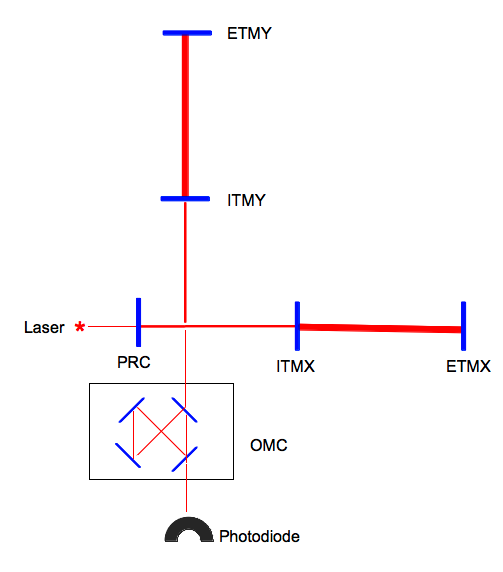
\includegraphics[width=\linewidth]{figures/theory/LIGO}
  \caption[Block diagram of LIGO]{
  \label{f:ligo}
Block diagram of LIGO, see the text for description.
}
\end{figure}%
The use of light actually simplifies the analysis, because the light
travels on null geodesics, so

\begin{equation*}
ds^2 = 0 = g_{\mu\nu} dx^\mu dx^\nu
\end{equation*}

We now consider a +-polarized gravitational wave travelling in the $z$
direction, and place the arms on the $x$ and $y$ axes.  We again
assume the frequency of the wave is large compared to the travel time
between the arms, which implies the, over the round trip, $h_+$ may be
taken to be constant and the metric becomes

\begin{equation*}
g_{\mu\nu} = -dt^2 + (1+h_+) dx^2 + (1-h_+) dy^2 + dz^2
\end{equation*}

Then for the $x$ axis, restoring physical units,

\begin{equation*}
c^2 dt^2 = (1+h_+) dx^2
\end{equation*}

and the round-trip travel time is

\begin{equation*}
t_x = \frac{2L}{c} \sqrt{1+h_+} \approx \frac{2L}{c} \left(1+\frac{h_+}{2} \right)
\end{equation*}

where we approximate the square root by its taylor series and ignore
higher-order terms in $h_+$.

Similarly the round-trip light travel time along the $y$ arm is

\begin{equation*}
t_y = \frac{2L}{c} \left(1-\frac{h_+}{2} \right)
\end{equation*}


Considering a single wavefront leaving the beam splitter, the
difference in return time is

\begin{equation*}
\Delta t = t_x - t_y = \frac{2L}{c} h_+
\end{equation*}

In interferometry what matters is not the difference in arrival time
of a wave front, but the difference in phase.  This difference will
cause an interference pattern that will serve as the readout.  If we
use laser light of frequency $f$ and wavelength $\lambda = c/f$ then a
time difference of $\Delta t$ corresponds to a phase difference of 

\begin{equation*}
\Delta \Phi = \frac{2\pi f}{\Delta t} = \frac{4\pi f L}{c} h_+
= \frac{4\pi L}{\lambda} h_+
\end{equation*}

As in the marble example, we can increase the sensitivity of the
instrument by increasing $L$, but practical considerations prevent us
from doing so.  One of these considerations is in fact the same for
marbles and light; the travel path must be in vacuum.  We
therefore employ the same trick and add two additional mirrors,
indicated as \texttt{ITMX} and \texttt{ITMY} (for ``initial test
masses'').  The addition of these mirrors creates a \emph{Fabry-Perot
cavity} in each arm.  By arranging the mirrors to be an integer
number of wavelengths apart a resonance is built up that can trap the
light for extended periods, approximately 200 bounces.  It can be seen
that if the mirrors are not appropriately spaced there will be
destructive interference between the light moving in different
directions.  As the power in the beam must be conserved, this results
in energy leaking out of the cavity, reducing the efficiency.

The addition of the Fabry-Perot cavities would suggest an increase in
phase difference of two orders of magnitude.  However, it is in fact
better than that.  The light is now in flight sufficiently long that,
for gravitational waves from astrophysical sources, $h_+$ will have
changed during the interval, and the above analysis is no longer
valid.  A more careful analysis shows that the improvement is on order
of three orders of magnitude.

In interferometry it is typically most useful to think of light as a
wave.  However, where in the toy example our ability to detect
gravitational waves was limited by our ability to count marbles in
real LIGO we are limited by our ability to count photons.  Photon
number is related to laser energy by $E=h\nu$, so we therefore want to
use as powerful a laser as possible.  There are, however, technical
obstacles to doing so.  In the latest LIGO run the laser power was up
to 14 W, although it was not always possible to run at this level.

In lieu of raising the laser power we can at least ensure that no
power is wasted.  LIGO is configured such that the beams interfere
destructively when they recombine, we say the instrument sits on a
\emph{dark fringe}~\footnote{Actually if we sat exactly on a dark
fringe then any change in the arm lengths would cause an increase of
light at the readout, and we would be unable to determine in which
direction the mirrors were moving.  We therefore sit a bit off the
dark fringe.}.  By conservation of energy all the power emitted by the
laser must go back towards the laser (neglecting the portion lost to
scattering, absorbed by the mirrors, etc).  We can recover this power
by adding another mirror, indicated on the diagram as \texttt{PRC}, or
power-recycling cavity.

The final feature on figure~\ref{f:ligo} is the \texttt{OMC} (output
mode cleaner), which was an important addition to the latest science
run.  A full description of this element is outside the scope of this
thesis, but we note briefly that the cross-section of a laser bean can
be decomposed into Hermite-Gaussian modes, as in
figure~\ref{f:hermite_gauss}.  The higher-order modes, being
non-symmetric, can induce angular instabilities in the mirrors.  It is
therefore advantageous to suppress such modes.

\begin{figure}
  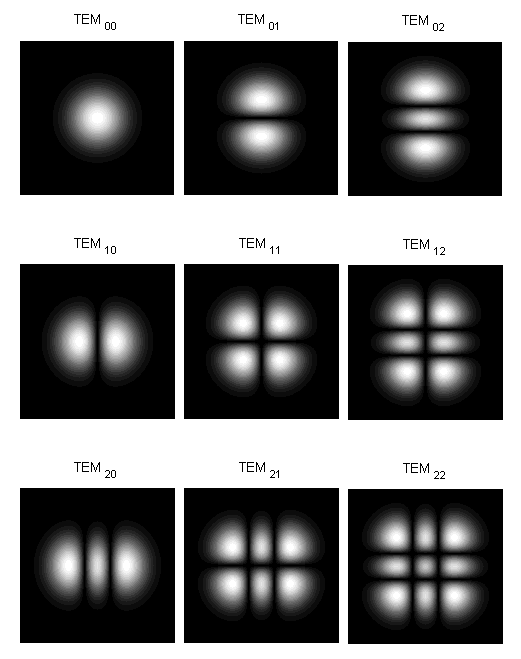
\includegraphics[width=\linewidth]{figures/theory/TEMmn}
  \caption[Laser modes]{
  \label{f:hermite_gauss}
Basis functions for the cross-sectional distribution of power in a
laser beam.  The lack of symmetry in the higher-order modes can induce
instabilities in the LIGO optics. (\it{Public-domain image taken from
Wikipedia}~\cite{wikipedia:temmn})
}
\end{figure}%

\subsection{Readout}

In order to operate correctly all the two Fabry-Perot cavities and the
power-recycling mirror must be positioned such that the light is
resonant.  The Michelson must likewise by arranged so that the output
photodetector is on a dark fringe.  When the instrument is in this
state we say it is \emph{locked}, at that point a gravitational wave
will perturb the system within limits and produce light out the
output.  However, the resonances must be very finely tuned and left
untouched the system would quickly fall out of lock due to random
motions of the mirrors.  There is therefore a need for continuous,
active corrections implemented by a system of sensors and servos
throughout the instrument.

Ignoring the OMC there are five degrees of freedom in
figure~\ref{f:ligo}: the two initial test masses, the two end masses,
and the PRC.  Each of these is individually measured and controllable.
However, it is more convenient to consider various linear combinations
of these degrees of freedom:

\begin{itemize}
\item \texttt{DARM}: the differential motion of the two end test masses
\item \texttt{CARM}: the common motion of the two end test masses
\item \texttt{MICH}: the differential motion of the ``small Michelson'' comprising
the ITMs and the beam splitter
\end{itemize}

One of the sensors used to keep the system on resonance is the output
photodector.  Along with this, note that \texttt{DARM} is the quantity
of interest in the experiment, the change in length produced by a
gravitational wave.    It turns outs that rather than reporting the
signal at the photodiode directly a better output is the degree to
which this degree of freedom is off the resonance condition, which is
recorded as \texttt{DARM\_ERR}.  Henceforth, and especially in
chapter~\ref{ch:detchar} we consider this ``the output of the
detector''.  It is not, however, the data stream in which we will
search for gravitational waves.  The detector output needs to be
calibrated with respect to the instrument's frequency response.  This
can be measured by injecting a sinewave of known amplitude into the
system by actuating one of the mirrors, and measuring the amplitude of
\darmerr.  The result is a complicated function of frequency.  This
can then be inverted to map \darmerr back to the true input, the
result is stored as \texttt{LSC\_STRAIN}, and it is that channel on
which gravitational wave searches are performed.

\subsection{Noise sources}

In addition to gravitational-wave sources the instrument is subject to
various other influences collectively known as noise.  These sources
are best characterized by their frequency profiles.

\begin{itemize} 

\item \emph{Seismic noise} is due to the coupling of the
instrument to the ground.  Much work has been been done, and much
research continues to be done, to isolate the mirrors from the
environment.  However, the isolation is not complete.  This noise
source dominates at low frequency, rising sharply above 40 Hz in
initial LIGO.  In advanced LIGO we hope to push this so-called
\emph{seismic wall} down to 10 Hz.  This noise source includes the
natural constant vibrations of the Earth, wind blowing over nearby
structures, and anthropogenic sources such as vehicles near the sites,
logging activity, etc.

\item \emph{Thermal noise}. Any system possesses energy proportional to 
the product of Boltzmann's constant and the ambient temperature.  The
energy manifests as random motion of the residual gas in the chambers,
the wires from which the mirrors are hung, and the mirrors themselves.
This produces noise that dominates from 40 Hz to approximately 200 Hz.

\item \emph{Shot noise} is the uncertainty inherent in counting
photons, as discussed above.

\end{itemize}

In addition to these broad-band sources of noise there are also
\emph{lines}, particular frequencies at which the noise is much
greater than the three sources above would produce.  Two of the most
significant are

\begin{itemize}
\item \emph{Electrical noise}.  Despite shielding, at 60 Hz there is a
sharp increase in the noise level due to the frequency of the US
electrical grid.
\item \emph{Violin modes}.  Although the wires suspending the mirrors
vibrate over a range of frequencies due to thermal noise, the
suspension system has a resonance at about $340 Hz$, producing much
more noise here.
\end{itemize}

There are also lines at higher harmonics of these frequencies.


\section{Conclusions}

In this chapter we reviewed the basic properties of gravitational
waves and the experiment to directly detect them.  In the next chapter
we extend the material in section~\ref{sec:general_relativity} to 
discuss how analytic and numeric methods are used to predict, in
detail, one form of gravitational radiation that is expected to be
seen by LIGO.



% Todo:
% Discuss the Weyl tensor, if needed for NR

